\documentclass[
11pt, % The default document font size, options: 10pt, 11pt, 12pt
%codirector, % Uncomment to add a codirector to the title page
]{charter} 


% El títulos de la memoria, se usa en la carátula y se puede usar el cualquier lugar del documento con el comando \ttitle
\titulo{Mejora del Sistema de Apunte Automático mediante la integración de IoT para monitoreo, control y gestión remota} 

% Nombre del posgrado, se usa en la carátula y se puede usar el cualquier lugar del documento con el comando \degreename
%\posgrado{Carrera de Especialización en Sistemas Embebidos} 
\posgrado{Carrera de Especialización en Internet de las Cosas} 
%\posgrado{Carrera de Especialización en Inteligencia Artificial}
%\posgrado{Maestría en Sistemas Embebidos} 
%\posgrado{Maestría en Internet de las cosas}

% Tu nombre, se puede usar el cualquier lugar del documento con el comando \authorname
% IMPORTANTE: no omitir titulaciones ni tildación en los nombres, también se recomienda escribir los nombres completos (tal cual los tienen en su documento)
\autor{Esp. Ing. William's Ernesto Limonchi Sandoval}

% El nombre del director y co-director, se puede usar el cualquier lugar del documento con el comando \supname y \cosupname y \pertesupname y \pertecosupname
\director{Mg. Ing. Juan Carlos Espinoza Guerra}
\pertenenciaDirector{Radio Observatorio de Jicamarca} 
\codirector{} % para que aparezca en la portada se debe descomentar la opción codirector en los parámetros de documentclass
\pertenenciaCoDirector{FIUBA}

% Nombre del cliente, quien va a aprobar los resultados del proyecto, se puede usar con el comando \clientename y \empclientename
\cliente{Dr. Danny Scipión}
\empresaCliente{Radio Observatorio de Jicamarca - IGP}
 
\fechaINICIO{08 de abril de 2025}		%Fecha de inicio de la cursada de GdP \fechaInicioName
\fechaFINALPlan{18 de junio de 2025} 	%Fecha de final de cursada de GdP
\fechaFINALTrabajo{15 de diciembre de 2025}	%Fecha de defensa pública del trabajo final


\begin{document}

\maketitle
\thispagestyle{empty}
\pagebreak


\thispagestyle{empty}
{\setlength{\parskip}{0pt}
\tableofcontents{}
}
\pagebreak


\section*{Registros de cambios}
\label{sec:registro}


\begin{table}[ht]
\label{tab:registro}
\centering
\begin{tabularx}{\linewidth}{@{}|c|X|c|@{}}
\hline
\rowcolor[HTML]{C0C0C0} 
Revisión & \multicolumn{1}{c|}{\cellcolor[HTML]{C0C0C0}Detalles de los cambios realizados} & Fecha      \\ \hline
0      & Creación del documento                                 &\fechaInicioName \\ \hline
%1      & Se completa hasta el punto 5 inclusive                & {día} de {mes} de 202X \\ \hline
%2      & Se completa hasta el punto 9 inclusive
%		  Se puede agregar algo más \newline
%		  En distintas líneas \newline
%		  Así                                                    & {día} de {mes} de 202X \\ \hline
%3      & Se completa hasta el punto 12 inclusive                & {día} de {mes} de 202X \\ \hline
%4      & Se completa el plan	                                 & {día} de {mes} de 202X \\ \hline

% Si hay más correcciones pasada la versión 4 también se deben especificar acá

\end{tabularx}
\end{table}

\pagebreak



\section*{Acta de constitución del proyecto}
\label{sec:acta}

\begin{flushright}
Buenos Aires, \fechaInicioName
\end{flushright}

\vspace{2cm}

Por medio de la presente se acuerda con el \authorname\hspace{1px} que su Trabajo Final de la \degreename\hspace{1px} se titulará ``\ttitle'' y consistirá en la implementar una mejora en el sistema actual que se tiene en el Radio Observatorio de Jicamarca. El trabajo tendrá un presupuesto preliminar estimado de 600 horas y un costo estimado de \$300, con fecha de inicio el \fechaInicioName\hspace{1px} y fecha de presentación pública el \fechaFinalName.

Se adjunta a esta acta la planificación inicial.

\vfill

% Esta parte se construye sola con la información que hayan cargado en el preámbulo del documento y no debe modificarla
\begin{table}[ht]
\centering
\begin{tabular}{ccc}
\begin{tabular}[c]{@{}c@{}}Dr. Ing. Ariel Lutenberg \\ Director posgrado FIUBA\end{tabular} & \hspace{2cm} & \begin{tabular}[c]{@{}c@{}}\clientename \\ \empclientename \end{tabular} \vspace{2.5cm} \\ 
\multicolumn{3}{c}{\begin{tabular}[c]{@{}c@{}} \supname \\ Director del Trabajo Final\end{tabular}} \vspace{2.5cm} \\
\end{tabular}
\end{table}




\section{1. Descripción técnica-conceptual del proyecto a realizar}
\label{sec:descripcion}

El Radio Observatorio de Jicamarca es una instalación de investigación científica gestionada por el Instituto Geofísico del Perú (IGP), reconocida mundialmente por sus estudios sobre la ionósfera. El sistema de apunte atuomático (ABS) fue diseñado originalmente para facilitar el cambio de apuntamiento de las antenas de manera manual o remota a través de Ethernet, asegurando la precisión requerida para estos experimentos. Sin embargo, a medida que los sistemas de monitoreo y gestión se han vuelto más sofisticados, ha surgido la necesidad de actualizar el sistema para mejorar la trazabilidad, mantenimiento y diagnóstico de fallos.

El proyecto consiste en la mejora del sistema ABS del Radio Observatorio de Jicamarca, un sistema crítico para el control de antenas utilizadas en experimentos avanzados sobre la ionósfera terrestre. Esta mejora tiene como objetivo modernizar el sistema integrando tecnologías de Internet de las Cosas (IoT) para permitir el monitoreo, control y gestión remota de las operaciones, ampliando sus capacidades actuales y optimizando la eficiencia en el manejo de datos.

Actualmente, el sistema permite el control remoto del apuntamiento de antenas, pero carece de capacidades avanzadas para el registro de datos, diagnóstico proactivo y monitoreo ambiental, lo que puede comprometer la confiabilidad y disponibilidad del sistema. La propuesta es implementar una solución IoT que no solo mantenga las funciones básicas del sistema, sino que también integre:

\begin{itemize}
	\item Monitoreo de variables ambientales como la temperatura para detectar condiciones adversas.
	\item Registro histórico de fallas y mantenimiento, mejorando la trazabilidad y análisis de fallos.
	\item Gestión de datos en tiempo real mediante una interfaz web multiplataforma.
	\item Desarrollo de shield personalizada para el monitoreo de temperatura.
\end{itemize}

El sistema propuesto incluye los siguientes componentes:
\begin{itemize}
    \item Microcontrolador TIVA TM4C1294 para control central.

	\item Shield personalizado para protección y expansión modular de sensores adicionales.

	\item Sensores ambientales, inicialmente de temperatura, con posibilidad de expansión.

	\item Servidor MQTT para comunicación eficiente y escalable.

	\item Base de datos local para almacenar y gestionar el historial de fallas y eventos.

	\item Aplicación web para acceso multiplataforma a datos y configuraciones.

	\item Seguridad en redes locales para garantizar acceso controlado.	
\end{itemize}

El diagrama en bloques del sistema se presenta en la Figura 1, donde se destacan los módulos de adquisición de datos, procesamiento, comunicación y visualización.

Las figuras se deben mencionar en el texto ANTES de que aparezcan con una frase como la siguiente: ``En la figura \ref{fig:diagBloques} se presenta el diagrama en bloques del sistema. Se observa que...''.  La regla es que las figuras nunca pueden ir antes de ser mencionadas en el texto, porque sino el lector no entiende por qué de pronto aparece una figura.

\begin{figure}[htpb]
	\centering 
	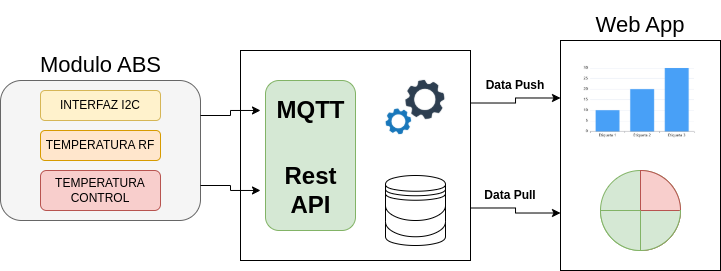
\includegraphics[width=.90\textwidth]{./Figuras/diagBloques.png}
	\caption{Diagrama en bloques del sistema.}
	\label{fig:diagBloques}
\end{figure}

\vspace{25px}


El tamaño del texto en TODAS las figuras debe ser adecuado \textbf{para que NO pase lo que ocurre en la figura \ref{fig:diagBloques}}, donde el lector debe esforzarse para poder leer el texto. 

Los colores usados en el diagrama deben ser adecuados, tal que ayuden a comprender mejor el diagrama. Se recomienda evitar colores primarios (como rojo, verde o cyan) y usar la gama de colores pastel.


\section{2. Identificación y análisis de los interesados}
\label{sec:interesados}

\begin{itemize}
	\item Auspiciante: es riguroso y exigente con la rendición de gastos. Tener mucho cuidado con esto.
	\item Cliente: el Radio Observatorio de Jicamarca, interesado en el desarrollo del proyecto para implementarlo en las mejoras de los futuros experimentos a realizar.
\end{itemize}


\begin{table}[ht]
%\caption{Identificación de los interesados}
%\label{tab:interesados}
\begin{tabularx}{\linewidth}{@{}|l|X|X|l|@{}}
\hline
\rowcolor[HTML]{C0C0C0} 
Rol           & Nombre y Apellido & Organización 	& Puesto 	\\ \hline
Auspiciante   & Radio Observatorio de     &    -          	&     -   	\\ \hline
Cliente       & \clientename      &\empclientename	& -       	\\ \hline
Impulsor      &                   &              	&        	\\ \hline
Responsable   & \authorname       & FIUBA        	& Alumno 	\\ \hline
Colaboradores &                   &              	&        	\\ \hline
Orientador    & \supname	      & \pertesupname 	& Director del Trabajo Final \\ \hline
Equipo        & - \newline 
				-          &   -           	&  -      	\\ \hline
Opositores    &                   &              	&        	\\ \hline
Usuario final &  Personal encargado en el sistema ABS           &              	&        	\\ \hline
\end{tabularx}
\end{table}

\section{3. Propósito del proyecto}
\label{sec:proposito}

El propósito de este proyecto es desarrollar una actualización integral del Sistema de Apunte Automático (ABS) del Radio Observatorio de Jicamarca, incorporando tecnologías de Internet de las Cosas (IoT) para mejorar su capacidad de monitoreo, control y gestión remota. Esta mejora permitirá un registro más detallado de datos operativos, diagnóstico de fallas en tiempo real y una interfaz de usuario más accesible y eficiente, optimizando así el rendimiento y la disponibilidad del sistema para las exigentes investigaciones científicas que se realizan en esta instalación.

\section{4. Alcance del proyecto}
\label{sec:alcance}

El alcance de este proyecto incluye el diseño, desarrollo y despliegue de una solución IoT para mejorar el Sistema de Apunte Automático (ABS) del Radio Observatorio de Jicamarca. Específicamente, se contempla:

\begin{itemize}
	\item La integración de un sensor de temperatura como variable inicial para monitoreo ambiental, con posibilidad de expansión para otros sensores en futuras etapas.

	\item El diseño y fabricación de un shield electrónico personalizado para protección y expansión modular del sistema, asegurando aislamiento eléctrico y compatibilidad con el microcontrolador TIVA TM4C1294.

	\item La migración del protocolo de comunicación actual hacia MQTT para mejorar la eficiencia, escalabilidad y gestión de datos.

	\item El desarrollo de una aplicación web multiplataforma para monitoreo y gestión del sistema, con almacenamiento local de datos históricos en contenedores Docker para mayor portabilidad y facilidad de mantenimiento.

	\item La implementación de medidas básicas de seguridad en red local para restringir el acceso no autorizado.

	\item Pruebas de funcionamiento y validación del sistema en condiciones reales en el Radio Observatorio de Jicamarca.
\end{itemize}

El presente proyecto no incluye:

\begin{itemize}
	\item El desarrollo de aplicaciones móviles nativas para iOS o Android.

	\item La implementación de algoritmos de inteligencia artificial o modelos predictivos para análisis de datos.

	\item La integración con servicios en la nube para almacenamiento remoto o procesamiento avanzado de datos.

	\item El rediseño físico o estructural del sistema de antenas o sus componentes mecánicos.

	\item El suministro de infraestructura de red, como switches, routers o fibra óptica.
\end{itemize}

\section{5. Supuestos del proyecto}
\label{sec:supuestos}

Para el desarrollo del presente proyecto se supone que:
\begin{itemize}
	\item El sistema actual del Radio Observatorio de Jicamarca está en condiciones operativas adecuadas para integrar las mejoras propuestas.

	\item El microcontrolador TIVA TM4C1294 es compatible con el shield personalizado y los sensores adicionales que se implementarán.

	\item Los sensores de temperatura y otros dispositivos de monitoreo estarán disponibles y serán compatibles con el entorno de operación del sistema ABS.

	\item El equipo de trabajo contará con acceso a las instalaciones del observatorio para pruebas, instalación y validación del sistema.

	\item El protocolo MQTT es adecuado para la transmisión de datos en el entorno local del observatorio, cumpliendo con los requisitos de latencia y estabilidad.

	\item Se dispondrá del conocimiento técnico para diseñar e implementar las interfaces de comunicación, el shield personalizado y el sistema de almacenamiento de datos.

	\item Las condiciones de red local serán suficientemente estables para permitir una conectividad constante entre el microcontrolador y el servidor de datos.

	\item No se prevén cambios regulatorios significativos que afecten el uso de tecnologías IoT en el ámbito de las telecomunicaciones del observatorio.

	\item Los recursos económicos y materiales necesarios para el diseño, fabricación y pruebas del shield personalizado estarán disponibles a lo largo del proyecto.
\end{itemize}

\section{6. Requerimientos}
\label{sec:requerimientos}

\begin{enumerate}
	\item Requerimientos funcionales:
	\begin{enumerate}
		\item El sistema debe permitir el monitoreo continuo de la temperatura en tiempo real. (Prioridad alta)
		\item El sistema debe registrar y almacenar eventos críticos, fallas y cambios de apuntamiento en una base de datos local. (Prioridad alta)
		\item El sistema debe permitir el control remoto del apuntamiento de antenas a través de una interfaz web multiplataforma. (Prioridad alta)
		\item El sistema debe enviar notificaciones de fallas a dispositivos conectados en la red local. (Prioridad media)
		\item La interfaz web debe ser compatible con navegadores modernos y adaptarse a dispositivos móviles. (Prioridad media)
		\item El sistema debe permitir la descarga de registros históricos en formato CSV o similar para análisis externo. (Prioridad media)
	\end{enumerate}
	\item Requerimientos de Hardware:
	\begin{enumerate}
		\item Uso de un microcontrolador TIVA TM4C1294 como núcleo del sistema. (Prioridad alta)
		\item Desarrollo de un shield electrónico personalizado para protección y expansión de sensores. (Prioridad alta)
		\item Inclusión de al menos un sensor de temperatura compatible con el microcontrolador. (Prioridad alta)
		\item  Fuente de alimentación y conversión de medios (fibra a Ethernet) para garantizar conectividad estable. (Prioridad alta)
	\end{enumerate}
	\item Requerimientos de Comunicación:
	\begin{enumerate}
		\item Implementación del protocolo MQTT para intercambio de datos entre el microcontrolador y los dispositivos conectados. (Prioridad alta)
		\item Configuración de un servidor MQTT local para la gestión de mensajes y datos en red cerrada. (Prioridad alta)
		\item Implementación de medidas básicas de seguridad para restringir el acceso no autorizado. (Prioridad alta)
	\end{enumerate}
	\item Requerimientos de Software:
	\begin{enumerate}
		\item Desarrollo de una aplicación web para gestión y visualización de datos. (Prioridad alta)
		\item Uso de contenedores Docker para facilitar la portabilidad y mantenimiento del servidor de datos. (Prioridad media)
		\item Compatibilidad con bases de datos locales para almacenamiento de históricos. (Prioridad alta)
	\end{enumerate}
	\item Requerimientos regulatorios y normativos:
	\begin{enumerate}
		\item Cumplimiento con las regulaciones locales de telecomunicaciones para transmisión de datos. (Prioridad alta)
		\item Asegurar que todos los componentes electrónicos cumplan con normas de seguridad eléctrica. (Prioridad alta)
		\item Cumplimiento con las normativas de protección de datos personales y privacidad en la red local. (Prioridad alta)
	\end{enumerate}
	\item Requerimientos opcionales:
	\begin{enumerate}
		\item Posibilidad de integración futura con algoritmos de inteligencia artificial para análisis predictivo. (Prioridad baja)
		\item Compatibilidad para agregar sensores adicionales, como humedad, presión o vibración. (Prioridad baja)
		\item Integración con servicios en la nube para acceso remoto en futuras etapas. (Prioridad baja)
	\end{enumerate}
\end{enumerate}

\section{7. Historias de usuarios (\textit{Product backlog})}
\label{sec:backlog}

\begin{enumerate}
	\item Como operador del sistema, quiero poder monitorear la temperatura en tiempo real para detectar condiciones adversas y evitar daños en los equipos.
	
	\textit{Story points}: 8 (complejidad: 3, dificultad: 2, incertidumbre: 3)
	
	\item Como ingeniero electrónico, quiero poder registrar y visualizar el historial de fallas para diagnosticar problemas rápidamente.
	
	\textit{Story points}: 10 (complejidad: 4, dificultad: 3, incertidumbre: 3)
	
	\item Como operador, quiero poder descargar los registros históricos para análisis detallado fuera de línea.
	
	\textit{Story points}: 7 (complejidad: 2, dificultad: 2, incertidumbre: 3)
	
	\item Como usuario del sistema, quiero acceder a la interfaz web desde cualquier dispositivo para monitorear y controlar las funciones del sistema de forma conveniente.
	
	\textit{Story points}: 9 (complejidad: 3, dificultad: 3, incertidumbre: 3)
	
\end{enumerate}

\section{8. Entregables principales del proyecto}
\label{sec:entregables}

Los entregables del proyecto son:

\begin{itemize}
	\item Manual de usuario.
	\item Diagrama de circuitos esquemáticos.
	\item Código fuente del firmware.
	\item Diagrama de instalación.
	\item Aplicación Web Multiplataforma.
	\item Base de datos local.
	\item Memoria del trabajo final.
\end{itemize}


\section{9. Desglose del trabajo en tareas}
\label{sec:wbs}

\begin{enumerate}
\item Diseño y Planificación del Sistema (51 hs)
	\begin{enumerate}
	\item Análisis de requisitos técnicos y funcionales. (10 hs)
	\item Diseño del shield personalizado. (15 hs) 
	\item Definición de arquitectura de hardware y software. (12 hs)
	\item Selección de sensores y componentes adicionales. (6 hs)
	\item Documentación inicial del proyecto. (8 hs)
	\end{enumerate}
\item Diseño general del proyecto (35 hs)
	\begin{enumerate}
	\item Realización de diagrama de bloques. (4 hs)
	\item Realización de diseño de la arquitectura del sistema. (4 hs)
	\item Obtener los componentes para el prototipo de pruebas. (12 hs)
	\item Diagrama de flujo del programa. (15 hs)
	\end{enumerate}
\item Desarrollo del Hardware (56 hs)
	\begin{enumerate}
	\item Diseño del esquemático del shield personalizado. (12 hs)
	\item Diseño y fabricación del PCB del shield. (35 hs)
	\item Montaje y soldadura de componentes. (9 hs)
	\end{enumerate}
\item Desarrollo del Firmware (127 hs)
	\begin{enumerate}
	\item Programación del microcontrolador TIVA TM4C1294. (25 hs)
	\item Implementación del protocolo MQTT. (22 hs)
	\item Desarrollo del código para manejo de sensores. (30 hs)
	\item Pruebas unitarias y depuración. (40 hs)
	\end{enumerate}
\item Desarrollo de Aplicación Web (180 hs)
	\begin{enumerate}
	\item Diseño de la interfaz de usuario. (20 hs)
	\item Programación del backend para gestión de datos. (35 hs)
	\item Integración con base de datos local. (20 hs)
	\item Programación del frontend para desarrollo de la aplicación Web. (40 hs)
	\item Integración entre el backend y frontend. (40 hs)
	\item Pruebas de funcionalidad y ajustes finales (25 hs)
	\end{enumerate}
\item Pruebas y Validación del Sistema (110 hs)
	\begin{enumerate}
	\item Pruebas de integración hardware-software. (40 hs)
	\item Pruebas de rendimiento del sistema en condiciones reales. (40 hs)
	\item Validación de comunicación y seguridad de datos. (30 hs)
	\end{enumerate}
\item Documentación y Entrega Final (20 hs)
	\begin{enumerate}
	\item Elaboración del manual de usuario. (6 hs)
	\item Documentación técnica del shield y firmware. (8 hs)
	\item Generación del informe final y memoria del proyecto. (6 hs)
	\end{enumerate}
\item Documentación y Entrega Final (29 hs)
	\begin{enumerate}
	\item Elaboración del manual de usuario. (6 hs)
	\item Documentación técnica del shield y firmware. (8 hs)
	\item Elaboración del manual para el desarrollador. (15 hs)
	\end{enumerate}
\item Presentación del trabajo (55 hs)
	\begin{enumerate}
	\item Elaborar la memoria técnica del trabajo final. (40 hs)
	\item Elaborar la presentación del trabajo final. (15 hs)
	\end{enumerate}
\end{enumerate}

Cantidad total de horas: 663 hs.
%\vspace{60px}


\section{10. Diagrama de Activity On Node}
\label{sec:AoN}

\begin{figure}[htpb]
	\centering 
	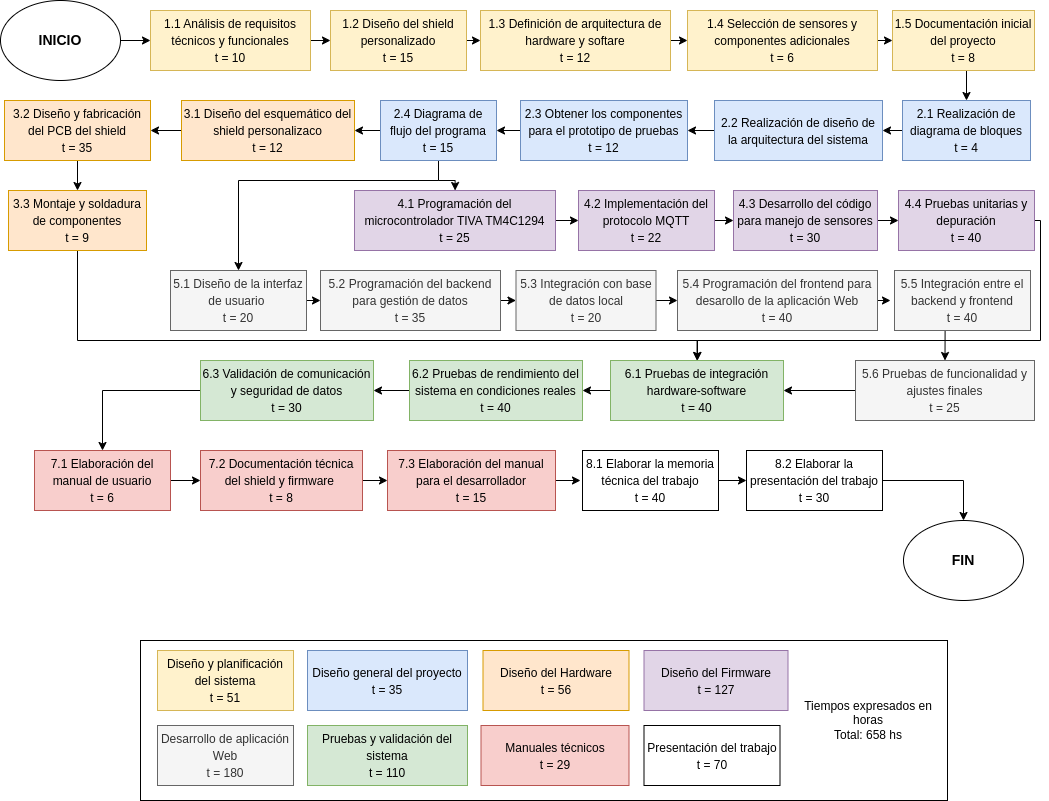
\includegraphics[width=1.0\textwidth]{./Figuras/AoN.png}
	\caption{Diagrama en Activity on Node.}
	\label{fig:AoN}
\end{figure}
\vspace{60px}
\section{11. Diagrama de Gantt}
\label{sec:gantt}

\begin{consigna}{red}
Existen muchos programas y recursos \textit{online} para hacer diagramas de Gantt, entre los cuales destacamos:

\begin{itemize}
\item Planner
\item GanttProject
\item Trello + \textit{plugins}. En el siguiente link hay un tutorial oficial: \\ \url{https://blog.trello.com/es/diagrama-de-gantt-de-un-proyecto}
\item Creately, herramienta online colaborativa. \\\url{https://creately.com/diagram/example/ieb3p3ml/LaTeX}
\item Se puede hacer en latex con el paquete \textit{pgfgantt}\\ \url{http://ctan.dcc.uchile.cl/graphics/pgf/contrib/pgfgantt/pgfgantt.pdf}
\end{itemize}

Pegar acá una captura de pantalla del diagrama de Gantt, cuidando que la letra sea suficientemente grande como para ser legible. 
Si el diagrama queda demasiado ancho, se puede pegar primero la ``tabla'' del Gantt y luego pegar la parte del diagrama de barras del diagrama de Gantt.

Configurar el software para que en la parte de la tabla muestre los códigos del EDT (WBS).\\
Configurar el software para que al lado de cada barra muestre el nombre de cada tarea.\\
Revisar que la fecha de finalización coincida con lo indicado en el Acta Constitutiva.

En la figura \ref{fig:gantt}, se muestra un ejemplo de diagrama de gantt realizado con el paquete de \textit{pgfgantt}. 
En la plantilla pueden ver el código que lo genera y usarlo de base para construir el propio.

Las fechas pueden ser calculadas utilizando alguna de las herramientas antes citadas. Sin embargo, el siguiente ejemplo
fue elaborado utilizando 
\href{https://docs.google.com/spreadsheets/d/1fBz8NhSpc4tkkhz3KjJCbh1nR_ltDkfEcZi4tZXduqs}{esta hoja de cálculo}.

Es importante destacar que el ancho del diagrama estará dado por la longitud del texto utilizado para las tareas 
(Ejemplo: tarea 1, tarea 2, etcétera) y el valor \textit{x unit}. Para mejorar la apariencia del diagrama, es necesario
ajustar este valor y, quizás, acortar los nombres de las tareas.

\begin{figure}[htpb]
  \begin{center}
    \begin{ganttchart}[
      time slot unit=day,
      time slot format=isodate,
      x unit=0.038cm,
      y unit title=0.7cm,
      y unit chart=0.6cm,
      milestone/.append style={xscale=4}
      ]{2021-03-05}{2021-12-16}
      \gantttitlecalendar*{2021-03-05}{2021-12-16}{year} \\
      \gantttitlecalendar*{2021-03-05}{2021-12-16}{month} \\
      \ganttgroup{Duración Total}{2021-03-05}{2021-12-16} \\
      %%%%%%%%%%%%%%%%%Organización
      \ganttgroup{Organización}{2021-03-05}{2021-04-16} \\
      \ganttbar{Planificación del proyecto}{2021-03-05}{2021-04-15} \\
      %%%%%%%%%%%%%%%%%Ejecución
      \ganttgroup{Ejecución}{2021-04-16}{2021-10-21} \\
      \ganttbar{Tarea 1}{2021-04-16}{2021-04-29} \\
      \ganttbar{Tarea 2}{2021-04-30}{2021-05-13} \\
      \ganttbar{Tarea 3}{2021-05-14}{2021-05-27} \\
      \ganttbar{Tarea 4}{2021-05-28}{2021-07-12} \\
      \ganttbar{Tarea 5}{2021-07-13}{2021-08-09} \\
      \ganttbar{Tarea 6}{2021-08-10}{2021-09-23} \\
      \ganttbar{Tarea 7}{2021-09-24}{2021-09-30} \\
      \ganttbar{Tarea 8}{2021-10-01}{2021-10-14} \\
      \ganttbar{Tarea 9}{2021-10-15}{2021-10-21} \\
      % %%%%%%%%%%%%%%%%%Finalización
      \ganttgroup{Finalización}{2021-10-22}{2021-12-16} \\
      \ganttbar{Memoria v1}{2021-10-22}{2021-11-04} \\
      \ganttbar{Memoria v2}{2021-11-05}{2021-11-18} \\
      \ganttbar{Memoria final}{2021-11-19}{2021-12-02} \\
      % La fecha del siguiente milestone es la fecha en que terminamos la memoria
      \ganttmilestone{Enviar memoria al director}{2021-12-02} \\
      \ganttbar{Elaborar la presentación}{2021-12-03}{2021-12-16} \\
      \ganttmilestone{Ensayo de la presentación}{2021-12-16} \\
      %%%%%%%%%%%%%%%%%%%%%%%%%%%%%%%%%%%%%%%%%%%%%%%%%%%%%%%%%%%%%%%
    \end{ganttchart}
  \end{center}
  \caption{Diagrama de gantt de ejemplo}
  \label{fig:gantt}
\end{figure}


\begin{landscape}
\begin{figure}[htpb]
\centering 
\includegraphics[height=.85\textheight]{./Figuras/Gantt-2.png}
\caption{Ejemplo de diagrama de Gantt (apaisado).} %Modificar este título acorde.
\label{fig:diagGantt}
\end{figure}

\end{landscape}

\end{consigna}


\section{12. Presupuesto detallado del proyecto}
\label{sec:presupuesto}

La moneda utilizada en el presupuesto es el dólar.

\begin{table}[htpb]
\centering
\begin{tabularx}{\linewidth}{@{}|X|c|r|r|@{}}
\hline
\rowcolor[HTML]{C0C0C0} 
\multicolumn{4}{|c|}{\cellcolor[HTML]{C0C0C0}COSTOS DIRECTOS} \\ \hline
\rowcolor[HTML]{C0C0C0} 
Descripción &
  \multicolumn{1}{c|}{\cellcolor[HTML]{C0C0C0}Cantidad} &
  \multicolumn{1}{c|}{\cellcolor[HTML]{C0C0C0}Valor unitario} &
  \multicolumn{1}{c|}{\cellcolor[HTML]{C0C0C0}Valor total} \\ \hline
Mano de obra  &
  \multicolumn{1}{c|}{663} & 
  \multicolumn{1}{c|}{\$ 4.00} &
  \multicolumn{1}{c|}{\$ 2652} \\ \hline
Sensor de temperatura &
  \multicolumn{1}{c|}{3} &
  \multicolumn{1}{c|}{\$ 5.00} &
  \multicolumn{1}{c|}{\$ 15.00} \\ \hline
Otros componentes &
\multicolumn{1}{c|}{1} &
   \multicolumn{1}{c|}{\$ 30.00} &
   \multicolumn{1}{c|}{\$ 30.00} \\ \hline
\multicolumn{3}{|c|}{SUBTOTAL} &
  \multicolumn{1}{c|}{\$ 2697} \\ \hline
\rowcolor[HTML]{C0C0C0} 
\multicolumn{4}{|c|}{\cellcolor[HTML]{C0C0C0}COSTOS INDIRECTOS} \\ \hline
\rowcolor[HTML]{C0C0C0} 
Descripción &
  \multicolumn{1}{c|}{\cellcolor[HTML]{C0C0C0}Cantidad} &
  \multicolumn{1}{c|}{\cellcolor[HTML]{C0C0C0}Valor unitario} &
  \multicolumn{1}{c|}{\cellcolor[HTML]{C0C0C0}Valor total} \\ \hline
30\% de costos dirctos  &
\multicolumn{1}{c|}{1} &
\multicolumn{1}{c|}{\$ 809.1} &
\multicolumn{1}{c|}{\$ 809.1} \\ \hline

\multicolumn{3}{|c|}{SUBTOTAL} &
\multicolumn{1}{c|}{\$ 809.1} \\ \hline
\rowcolor[HTML]{C0C0C0}
\multicolumn{3}{|c|}{TOTAL} &
\multicolumn{1}{c|}{\$ 3506.1} \\ \hline
\end{tabularx}%
\end{table}


\section{13. Gestión de riesgos}
\label{sec:riesgos}

 
Riesgo 1: fallo en el microcontrolador TIVA TM4C1294
\begin{itemize}
	\item Severidad (S): 9 \\ 
	El sistema depende completamente del microcontrolador para el control de antenas y gestión de datos, por lo que su fallo implica una pérdida crítica de funcionalidad.
	\item Probabilidad de ocurrencia (O): 3 \\
	Los microcontroladores TIVA son altamente confiables, pero pueden fallar por sobrecargas, errores de diseño del shield o daños físicos.
\end{itemize}   

Riesgo 2: interferencia en la comunicación MQTT
\begin{itemize}
	\item Severidad (S): 8 \\ 
	Una falla en la comunicación puede dejar el sistema sin datos críticos y dificultar el monitoreo remoto.
	\item Probabilidad de ocurrencia (O): 3 \\
	Las redes locales pueden experimentar interferencias o congestión, especialmente en ambientes con alta demanda de ancho de banda.
\end{itemize}   

Riesgo 3: daño físico al shield personalizado
\begin{itemize}
	\item Severidad (S): 7 \\ 
	Un daño en el shield puede comprometer la protección eléctrica del sistema y generar fallos críticos.
	\item Probabilidad de ocurrencia (O): 4 \\
	El proceso de soldadura y montaje conlleva riesgos si no se toman las precauciones adecuadas.
\end{itemize}   

Riesgo 4: fallo en los sensores de temperatura
\begin{itemize}
	\item Severidad (S): 6 \\ 
	Los datos de temperatura son importantes para evitar sobrecalentamientos y daños en los equipos.
	\item Probabilidad de ocurrencia (O): 6 \\
	Los sensores son componentes relativamente sensibles que pueden dañarse por picos de voltaje o condiciones ambientales extremas.
\end{itemize}   

Riesgo 5: problemas de seguridad en la red local
\begin{itemize}
	\item Severidad (S): 10 \\ 
	Una brecha de seguridad puede exponer información sensible y comprometer la estabilidad del sistema.
	\item Probabilidad de ocurrencia (O): 5 \\
	Aunque se planea implementar medidas básicas de seguridad, siempre existe el riesgo de ataques externos o internos.
\end{itemize}   



b) Tabla de gestión de riesgos: (El RPN se calcula como RPN=SxO)

\begin{table}[htpb]
\centering
\begin{tabularx}{\linewidth}{@{}|X|c|c|c|c|c|c|@{}}
\hline
\rowcolor[HTML]{C0C0C0} 
Riesgo & S & O & RPN & S* & O* & RPN* \\ \hline
     1 & 9 & 3 &  27 &    &    &      \\ \hline
     2 & 8 & 3 &  24 &    &    &      \\ \hline
     3 & 7 & 4 &  28 &    &    &      \\ \hline
     4 & 6 & 6 &  36 &    &    &      \\ \hline
     5 & 10 & 5 & 50 &    &    &      \\ \hline
\end{tabularx}%
\end{table}

Criterio adoptado: 

Se tomarán medidas de mitigación en los riesgos cuyos números de RPN sean mayores a 30

Nota: los valores marcados con (*) en la tabla corresponden luego de haber aplicado la mitigación.

c) Plan de mitigación de los riesgos que originalmente excedían el RPN máximo establecido:
 
Riesgo 4: Implementar redundancia de sensores en puntos críticos para validar las mediciones.
  \begin{itemize}
	\item Severidad (S): 6 \\ 
	Los datos de temperatura son importantes para evitar sobrecalentamientos y daños en los equipos.
	\item Probabilidad de ocurrencia (O): 2 \\
	La probabilidad de ocurrencia es baja, porque 
	\end{itemize}


\section{14. Gestión de la calidad}
\label{sec:calidad}

\begin{consigna}{red}
Elija al menos diez requerimientos que a su criterio sean los más importantes/críticos/que aportan más valor y para cada uno de ellos indique las acciones de verificación y validación que permitan asegurar su cumplimiento.

\begin{itemize} 
\item Req \#1: copiar acá el requerimiento con su correspondiente número.

\begin{itemize}
	\item Verificación para confirmar si se cumplió con lo requerido antes de mostrar el sistema al cliente. Detallar.
	\item Validación con el cliente para confirmar que está de acuerdo en que se cumplió con lo requerido. Detallar. 
\end{itemize}

\end{itemize}

Tener en cuenta que en este contexto se pueden mencionar simulaciones, cálculos, revisión de hojas de datos, consulta con expertos, mediciones, etc.  

Las acciones de verificación suelen considerar al entregable como ``caja blanca'', es decir se conoce en profundidad su funcionamiento interno.  

En cambio, las acciones de validación suelen considerar al entregable como ``caja negra'', es decir, que no se conocen los detalles de su funcionamiento interno.

\end{consigna}

\section{15. Procesos de cierre}    
\label{sec:cierre}

\begin{consigna}{red}
Establecer las pautas de trabajo para realizar una reunión final de evaluación del proyecto, tal que contemple las siguientes actividades:

\begin{itemize}
	\item Pautas de trabajo que se seguirán para analizar si se respetó el Plan de Proyecto original:\\
	 - Indicar quién se ocupará de hacer esto y cuál será el procedimiento a aplicar. 
	\item Identificación de las técnicas y procedimientos útiles e inútiles que se emplearon, los problemas que surgieron y cómo se solucionaron:\\
	 - Indicar quién se ocupará de hacer esto y cuál será el procedimiento para dejar registro.
	\item Indicar quién organizará el acto de agradecimiento a todos los interesados, y en especial al equipo de trabajo y colaboradores:\\
	  - Indicar esto y quién financiará los gastos correspondientes.
\end{itemize}

\end{consigna}

\end{document}